% Following magic comments allow for compilation of root file
% !TEX root = ../../../../temp_manuscript.tex

\chapter{Introduction}

\begin{ChapterAbstractNoTitle}
Sora recently visited his doctor because he had constant headaches, often felt nauseous, and had blurry vision.
His doctor referred him to the hospital, where he came under the care of Egwene, a neuro-oncologist, who explained to him that he might have a brain \gls{tumor} and that she wanted to make a scan of his brain.
Shocked and a bit worried by this news, Sora went into the MRI scanner, which he was told could make an image of the \gls{tumor} inside his head.
At the same time Sora was getting out of the scanner, his scans were being analyzed by a computer that could pick up on details of the scan invisible to the human eye.
The computer used these scan details to determine several \gls{tumor} characteristics related to the aggressiveness of the \gls{tumor}.
A couple of minutes later, Sora walked back into the office of Egwene, who had already looked at the scans and the \gls{tumor} characteristics provided by the computer.
Based on Egwene's experience with these \glspl{tumor} and the information provided by the computer, she could comfort Sora and tell him that the \gls{tumor} did not seem to be very aggressive.
Together they discussed possible treatment options and the best course of action from here on out.
By analyzing the scan using a computer directly after the scan was made, Sora could go home without worrying about the results of his scan, and Egwene could rest assured knowing that she could optimally tailor the treatment to Sora's specific situation.
\end{ChapterAbstractNoTitle}

Although the above story is currently (unfortunately) still fictional, research in medical imaging has rapidly evolved over the last couple of years, bringing the existence of such automated systems closer to reality than ever before.
However, there is still a gap to bridge before they can find their way into the clinic.
Therefore, in this thesis, I focus on automated systems that analyze \acrshort{MRI} scans of glioma patients and provide clinicians with additional information earlier in the clinical decision making process, enabling them to provide care that is more personalized to each patient.

\section{Glioma}

When cells reproduce, genetic mutations can occur that result in the cells starting to grow uncontrollably.
This uncontrollable growth of new cells is commonly known as cancer.
When the cancerous cells lump together, the single mass that they form is called a \gls{tumor}.
\Glspl{tumor} can originate from and occur almost everywhere in the human body, and the location where the \gls{tumor} occurs is not always the same as the location from which the cancerous cells originate.
When the cancerous cells form a \gls{tumor} in the location from which they originate, the \gls{tumor} is called a primary \gls{tumor}.
Hence, primary brain \glspl{tumor} are \glspl{tumor} located in the brain that are formed by cells that mutated from (healthy) brain cells.

Since different types of brain cells exist, the cancerous cells can have mutated from these different cells.
Therefore, primary brain \glspl{tumor} are categorized by the type of brain cells from which they mutated, with \glspl{glioma} being the most prevalent \autocite{leece2017indicence}.
\Glspl{glioma} are \glspl{tumor} which cancerous cells mutated from \glspl{gcell}.
\Glspl{gcell}, which play a supporting role in the \acrlong{CNS}, are the most abundant cell type in the brain \autocite{jakel2017glial}.
Although \gls{glioma} have a low incidence compared to other cancers, around \per{1.7} globally \autocite{leece2017indicence}, they are one of the deadliest with a median survival of nine months in the worst case to fifteen years in the best case \autocite{ho2014incidence, olar2015survival}.
Unfortunately, no cure exists for \gls{glioma} but there are several treatments that can prolong the life expectancy and/or quality of life of patients.
Since no two \gls{glioma} are the same, the treatment is tailored to each specific case in order to deliver the best possible treatment for each patient.
Therefore, it is important to categorize \gls{glioma} in a clinically relevant way, which supports the clinical decision making process and leads to better patient care.

\section{Categorization of glioma}
Historically \glspl{glioma} were categorized based solely on their histopathological appearance, that is, the appearance of the \gls{tumor} cells under a microscope.
Up to 2016, the \gls{WHO} recognized four different types of \gls{glioma}: \gls{astro}, \gls{oliastro}, \gls{oli}, and \gls{GBM} (since 2016 known as just \gls{glioblastoma}) \footnote{For readers unfamiliar with the newly introduced terms, a glossary is available on page \pageref{glossary} as a reference.}.
This classification depended on the type of \glspl{gcell} that were visible in the \gls{tumor} tissue \autocite{louis2007who}.
Classifying \gls{glioma} based on their \gls{gcell} type is often called typing.
In addition to \gls{glioma} typing, \glspl{tumor} were assigned a grade to indicate their aggressiveness; this process is referred to as grading.
The grade was either II, III, or IV, with a grade IV \gls{glioma} being the most aggressive.
Although grade I \gls{glioma} exist, these are regarded as benign and as such are excluded from further consideration in this thesis.
Historically, grade II \gls{glioma} were often referred to as \gls{LGG}, and grade III and grade IV \gls{glioma} were referred to as \gls{HGG}.
There is some relation between the type and grade of a glioma; \gls{glioblastoma} are grade IV glioma, the most aggressive type, while \gls{astro}, \gls{oliastro}, and \gls{oli} are less aggressive and can be either grade II or grade III \footnote{Officially \gls{glioblastoma} are grade IV \gls{astro}, however in practice these are always referred to as \gls{glioblastoma}, while \gls{astro} refers to the grade II/III ones.}.

This categorization based on the typing and the grading of the \gls{tumor} is suboptimal.
Firstly, the histopathological categorization and grading of the \glspl{tumor} are very observer-dependent \autocite{mittler1996gradingreliability, vandenbent2010interobserver}.
Since the clinical decision making depended on the categorization, this observer dependency could lead to an inadequate treatment of the \gls{tumor} \autocite{vandenbent2010interobserver}.
Secondly, within these categories, large differences between the survival of patients existed  \autocite{dubbink2015molecular}.
This suggests a different underlying mechanism that determines the aggressiveness of the \gls{tumor} than what the categorization based on grade and type accounts for.
For example, some grade II and grade III \gls{glioma} showed survival rates more characteristic of grade IV \gls{glioma} than other grade III \gls{glioma}.
It was found that this difference in survival can be better explained by the genetic features of the \gls{tumor} \autocite{dubbink2015molecular,eckel2015gliomagroups}.
Therefore, in 2016 the \gls{WHO} updated the categorization of \gls{glioma} to include these genetic features and depend less on the histopathology alone \cite{louis20162016}.
This update led to better patient stratification and more objective categorization of \gls{glioma} \autocite{molinaro2019geneticepidemiology}.
An overview of the \gls{WHO} 2016 guidelines and their relation to the previous guidelines is presented in \cref{fig:intro_glioma_categorization}.

\begin{figure}[hbt]
    \resizebox{0.98\textwidth}{!}{\subimport{Figures/}{WHO_2016_flowchart.pgf}}
    \centering
    \caption{The \acrfull{WHO} 2016 categorizaton of glioma. The aggressiveness of the \glspl{tumor} increases from left to right}\label{fig:intro_glioma_categorization}
\end{figure}

In the updated guidelines, the \gls{glioma} typing has become less relevant.
The histopathology now only needs to distinguish (what where historically) \gls{astro} and \gls{oli} (\gls{LGG}) on the one hand and \gls{glioblastoma} (\gls{HGG}) on the other hand.
with the introduction of the 2016 guidelines, the definition of \gls{LGG} and \gls{HGG} also changed; grade III \gls{glioma} are now often considered \gls{LGG} instead of \gls{HGG}.
However, this categorization is still a topic of debate and guidelines are continuously updated as new evidence on better categorizations becomes available \autocite{lous2020impactnow}.
In this thesis, grade II and III \gls{glioma} are considered \gls{LGG} and grade IV \gls{glioma} are considered \gls{HGG}, in accordance with \gls{WHO} 2016 guidelines.
The new guidelines no longer recognize \glspl{oliastro}; instead \gls{LGG} can now only be either \gls{astro} or \gls{oli}.
This greatly reduces the observer variability as the genetic features are more clearly defined than the histopathological features.
Further categorization of the \gls{glioma} is now based on two genetic features:  the \gls{IDHmut} and \gls{codeletion}.
% Needed to correctly use IDH abbrv
\glsunset{IDH}
These are two genetic features that occur at specific parts of the genome but only occur in the genome of the \gls{tumor} and not in the genome of the healthy tissue.
When the \gls{IDH} gene is normal (the same as the \gls{IDH} gene of the healthy tissue), the \gls{tumor} is referred to as \gls{IDH} wildtype.
If the \gls{IDH} gene is mutated from the normal gene, the \gls{tumor} is an \gls{IDH} mutated \gls{tumor}.
The same holds for the \gls{codeletion}: if it is the same as the original chromosome it is \acl{1p19qint}, if it mutated from the original it is \acl{1p19qcodel}.

Within the \gls{LGG} (what was previously \gls{astro}, \gls{oliastro}, and \gls{oli}), the following categories now exist:
\begin{itemize}
    \item Diffuse \gls{astro}, \gls{IDH} wildtype
    \item Diffuse \gls{astro}, \gls{IDH} mutated and \acl{1p19qint}
    \item \Gls{oli}, \gls{IDH} mutated and \acl{1p19qcodel}
\end{itemize}
No category exists for \gls{IDH} wildtype, \acl{1p19qcodel} \gls{glioma} as it was found that all \acl{1p19qcodel} \glspl{tumor} are also \gls{IDH} mutated \autocite{labussi20101p19qcodeletedIDH}.
Although the terms \gls{astro} and \gls{oli} are still used in the updated guidelines, they no longer carry the same meaning as before, since their categorization is no longer based on the \gls{gcell} type but instead on the genetic features.
Among the \gls{LGG}, the \glspl{oli} have the best prognosis and the diffuse \glspl{astro} \gls{IDH} wildtype show the worst prognosis \autocite{eckel2015gliomagroups}.
Due to the aggressiveness of \gls{IDH} wildtype \gls{astro}, it is even suggested that these are actually misclassified \gls{glioblastoma} \autocite{hartmann2010IDH1gbm, brat2018IMPACT}.




The \gls{WHO} 2016 guidelines also categorize \gls{glioblastoma} based on the \gls{IDHmut} status, where \gls{IDH} mutated \gls{glioblastoma} have a better prognosis than \gls{IDH} wildtype \gls{glioblastoma}.
Although the guidelines currently only include the \gls{IDHmut} status for the categorization of \gls{HGG}, there is another genetic feature that plays an important role in \gls{glioblastoma}: \gls{MGMTmet}.
% Needed to correctly use the MGMT abbrv
\glsunset{MGMT}
Patients with \gls{MGMT} methylated \glspl{tumor} survive longer than patients with \gls{MGMT} unmethylated \glspl{tumor} \autocite{martinez2007MGMT, gessler2018MGMT, weller2009molecularGBM}.
Thus, although not used for \gls{glioma} typing, the \gls{MGMT} methylation status is often relevant for the clinical decision making \autocite{molinaro2019geneticepidemiology}.

Not only do the genetic features determine the aggressiveness of the \gls{tumor}, but they also influence the \gls{tumor}'s response to certain treatments.
For example \gls{IDH} mutated \gls{glioma} respond better to radiotherapy than \gls{IDH} wildtype \gls{glioma} \autocite{juratli2015IDHtreatment}, and the \gls{codeletion} status and \gls{MGMT} methylation status might be predictors of the \gls{tumor}'s sensitivity to chemotherapy \autocite{idbaih2007markersresponse}.
Thus, it is important to know the genetic features of a \gls{glioma}, both for the prognosis of the patient and for deciding on the most suitable treatment.

In current clinical practice, the genetic and histopathological features are determined from \gls{tumor} tissue obtained through biopsy or resection.
In the case of a biopsy, a small part of the \gls{tumor} is removed for analysis to decide on the further treatment of the \gls{tumor}.
Thus, biopsies are not part of the treatment but are merely used to decide on further treatment options.
Resection is part of the treatment process and involves surgically removing as much of the \gls{tumor} as possible.
Part of the removed \gls{tumor} can then be used for the genetic and histopathological analysis to decide on follow-up treatments, such as chemotherapy and radiotherapy.
Taking a biopsy or resecting the \gls{tumor} requires intrusive surgery, which not only puts an extra burden on the healthcare system but also comes with risks for the patient \autocite{chen2009biopsy}.
Therefore, it would be beneficial if the genetic features of a \gls{glioma} can be determined without the need for a biopsy of which the sole purpose of the biopsy is to obtain tissue that can be analyzed to help the clinical decision making.

A non-invasive method to determine the genetic features of the \gls{tumor} not only obviates the need for an intrusive surgical operation, but it can also provide relevant information earlier in the treatment process, which can aid in the clinical decision making.
In the case of an asymptomatic \gls{tumor} with a favorable genetic profile a watch-and-wait approach may be considered since leaving the \gls{tumor} untreated might have less of a negative impact than the potentially damaging effect of the treatment on the healthy tissue \autocite{vandenbent2012lggtreatment, welle2017EANO}.
Since \gls{MRI} is already part of the standard clinical pathway for glioma patients, it is the ideal candidate for a non-invasive way of identifying the genetic and histopathological features of the \gls{tumor}.

\section{MRI analysis of glioma}

\Acrfull{MRI} is an imaging technique that uses the magnetic properties of protons, one of three elementary particles that form an atom, to create an image.
Although protons appear in all atoms, hydrogen atoms are of particular interest because they consist of a single proton, simplifying their magnetic properties and thus making them easier to use in the imaging process.
Furthermore, a water molecule contains two hydrogen atoms and since the majority of the human body consists of water, hydrogen atoms (and thus protons) are abundant in the human body, especially in soft tissue.
An \gls{MRI} scanner manipulates the protons to form an image and can even manipulate them in different ways to obtain different imaging contrasts.
An example of an \gls{MRI} scanner is shown in \cref{fig:intro_MR_machine}.


\begin{figure}[hbt]
    \includegraphics[width=\textwidth]{Figures/MRI_scanner.jpg}
    \caption{A \acrfull{MRI} scanner}\label{fig:intro_MR_machine}
\end{figure}

\gls{MRI} is routinely used in clinical care to distinguish between healthy and diseased tissue and to characterize the type of diseased tissue.
Shortly after the first introduction of \gls{MRI}, it was proposed that the method could be used to identify \glspl{tumor} \autocite{damadian1971tumor}.
After some improvements, the technique was first applied to the brain in 1980 \autocite{holland1980brain}, and in the same year MRI was first used to investigate a brain \gls{tumor} \autocite{hawkes1980NMRbrain}.
Since then, the quality of \gls{MRI} scans has vastly improved and \gls{MRI} techniques have been developed that can image various tissue characteristics.
Some examples of \gls{MRI} scans are shown in \cref{fig:intro_MR_example}, showing the different tissue characteristics, although many more techniques to image other tissue characteristics exist.
In these scans, the \gls{tumor} can clearly be seen, which gives the clinician important information in a non-invasive way, with minimal risk for the patient.
Therefore, \gls{MRI} is part of the standard-of-care for brain \gls{tumor} diagnosis and treatment decisions.

\begin{figure}[hbt]
    \centering
    \begin{subfigure}[b]{0.45\textwidth}
        \centering
        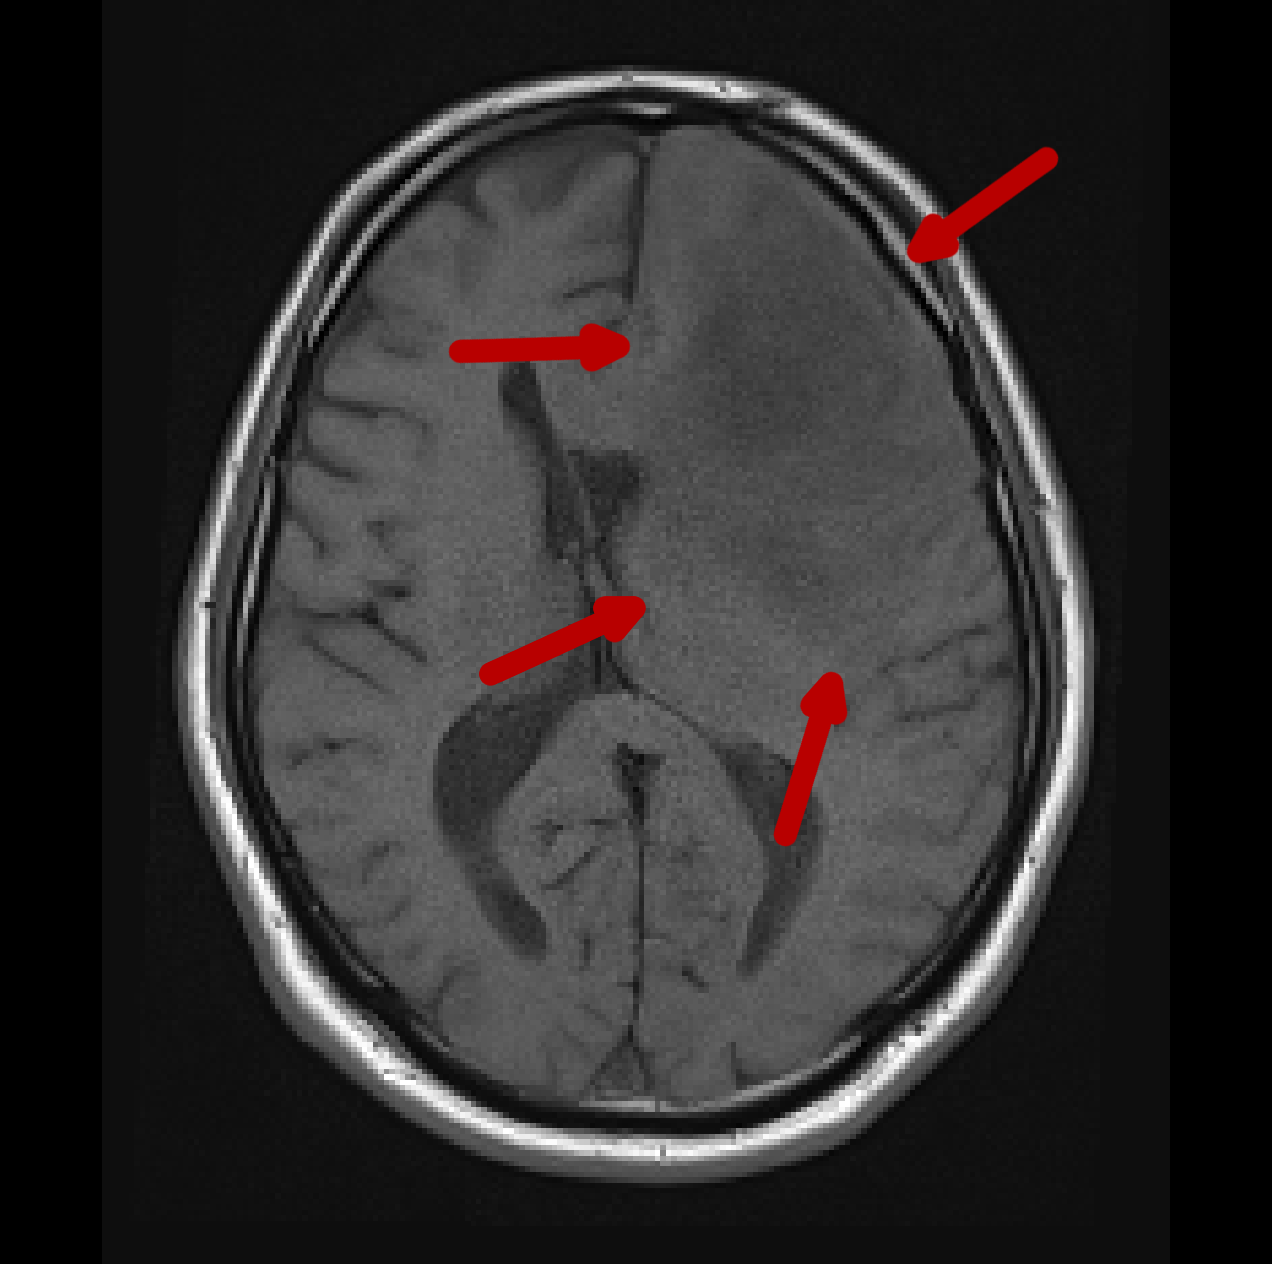
\includegraphics[width=\textwidth]{Figures/T1_arrows.png}
        \caption{Pre-contrast T1-weighted scan}\label{fig:intro_T1}
    \end{subfigure}
    \begin{subfigure}[b]{0.45\textwidth}
        \centering
        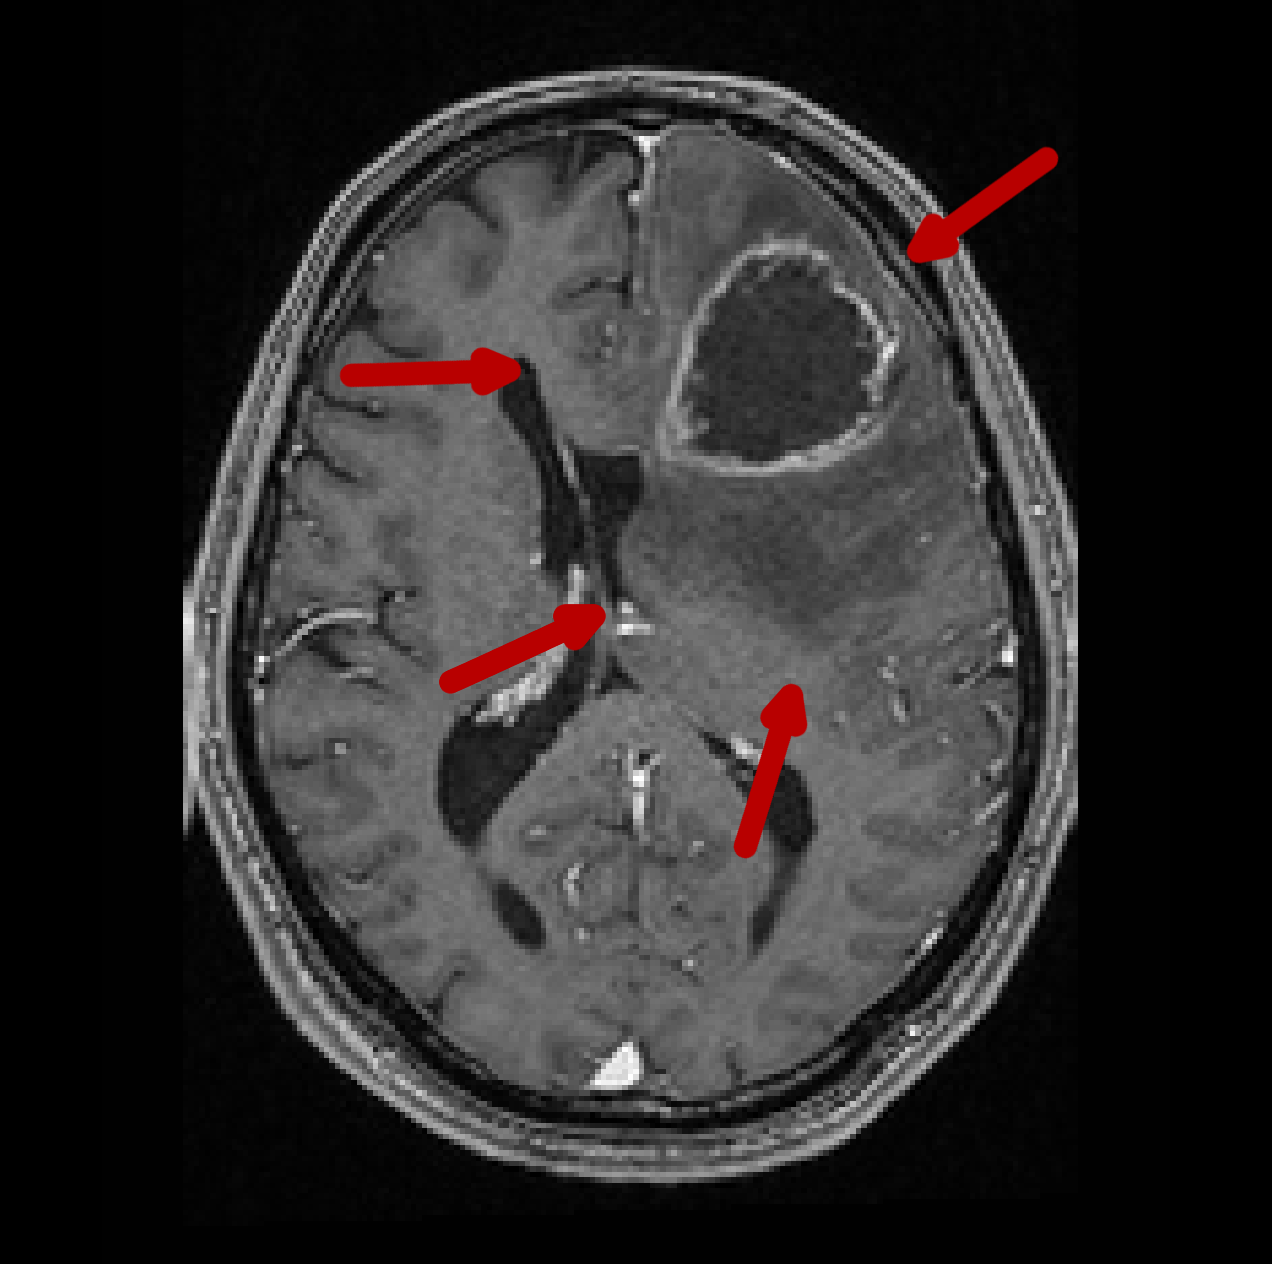
\includegraphics[width=\textwidth]{Figures/T1GD_arrows.png}
        \caption{Post-contrast T1-weighted scan}\label{fig:intro_T1GD}
    \end{subfigure}

    \begin{subfigure}[b]{0.45\textwidth}
        \centering
        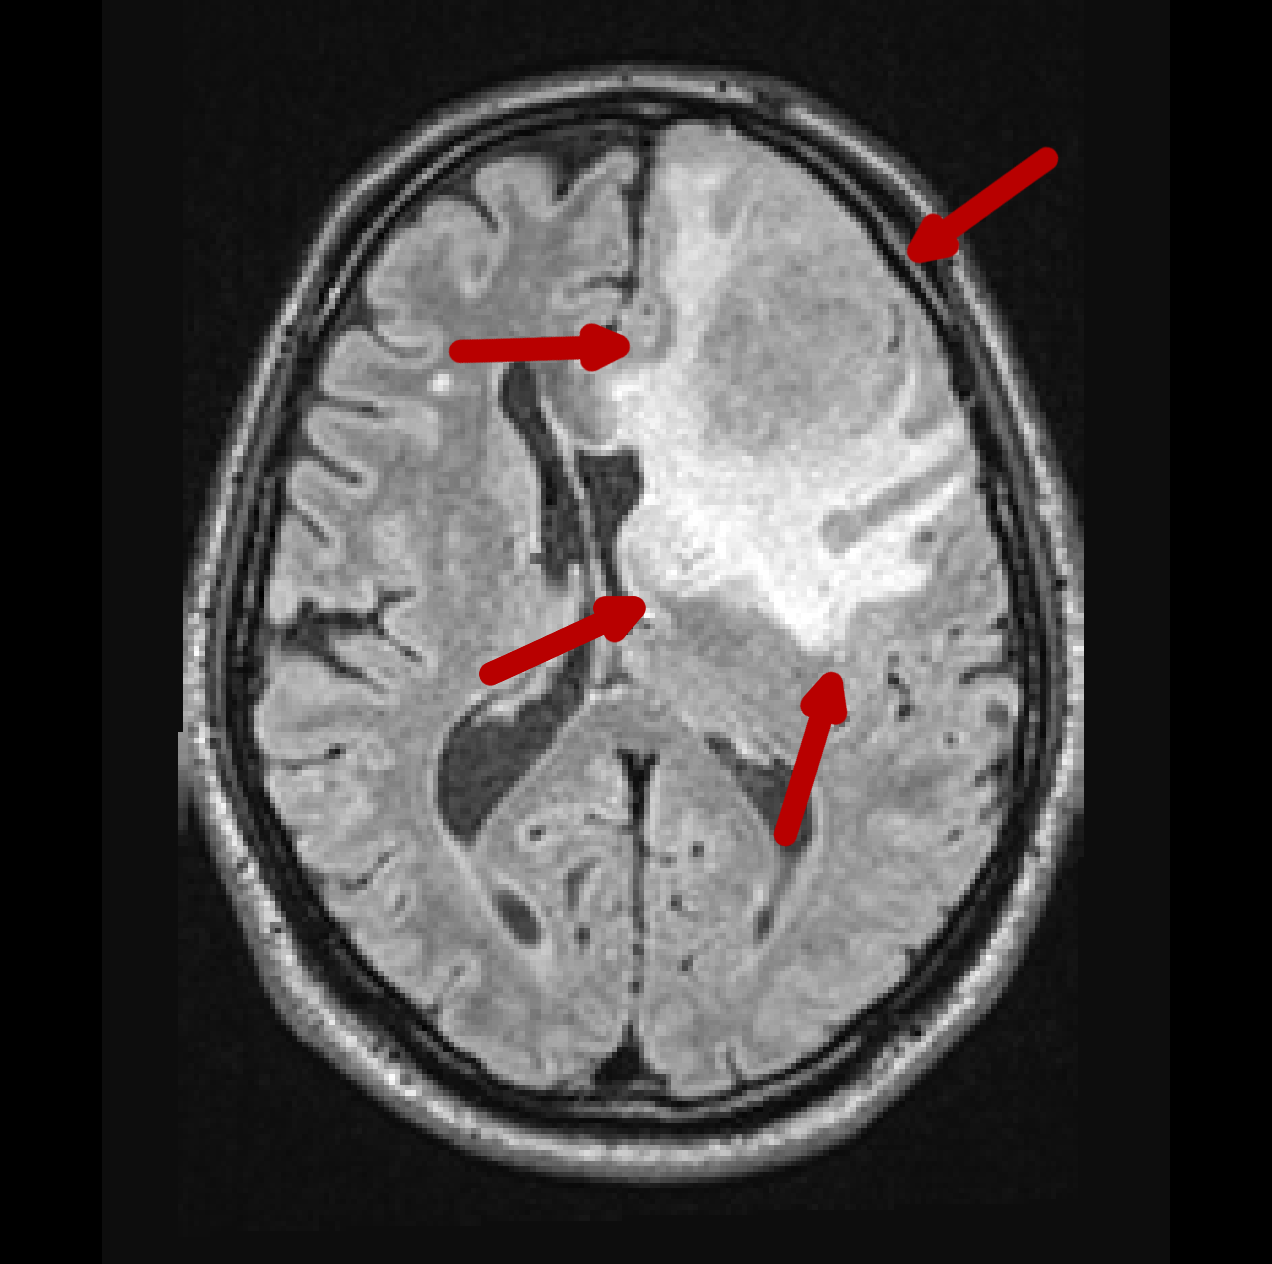
\includegraphics[width=\textwidth]{Figures/FLAIR_arrows.png}
        \caption{T2-weighted FLAIR scan}\label{fig:intro_FLAIR}
    \end{subfigure}
    \begin{subfigure}[b]{0.45\textwidth}
        \centering
        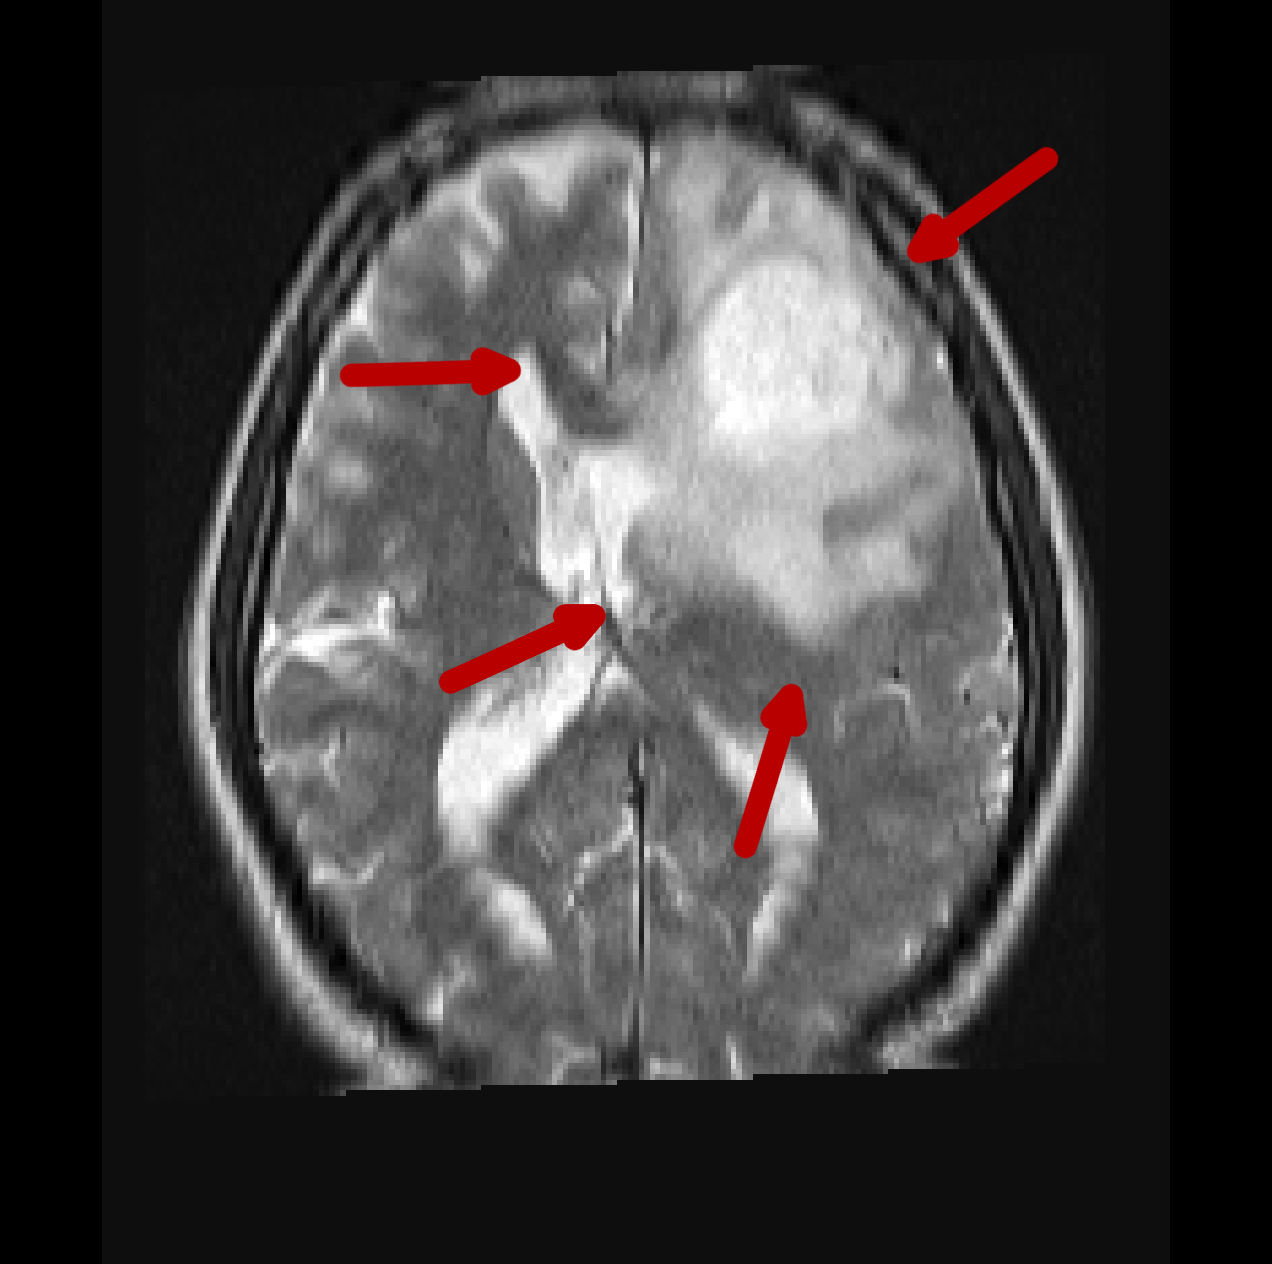
\includegraphics[width=\textwidth]{Figures/T2_arrows.png}
        \caption{T2-weighted scan}\label{fig:intro_T2}
    \end{subfigure}

    \caption{Examples of \acrshort{MRI} scans with different contrasts, the red arrows point to the \gls{tumor}.
    On some scans (\textbf{\protect\subref{fig:intro_T1}}, \textbf{\protect\subref{fig:intro_T1GD}}) the \gls{tumor} appears darker than the surrounding healthy tissue, whereas on others (\textbf{\protect\subref{fig:intro_FLAIR}}, \textbf{\protect\subref{fig:intro_T2}}) it appears as a bright lump.
     The different imaging contrasts provide clinically relevant information of the glioma; for example, the fact that scan \textbf{\protect\subref{fig:intro_T1GD}} shows a bright ring around a dark center suggests that this is a glioblastoma}\label{fig:intro_MR_example}
\end{figure}

\gls{MRI} scans are already routinely being used to get a first indication of the aggressiveness of the \gls{tumor}, mainly for \gls{tumor} grading \autocite{upadhyay2011MRIevaluation}.
With the increasing importance of genetic features of the \glspl{tumor}, research has focused on identifying imaging markers that correlate with an underlying physiological aspect, in this case the genetic features of a \gls{tumor} \autocite{patel2017mismatch, smits2016imaging}.
The presence of these imaging markers in \gls{MRI} scans proves the potential of \gls{MRI} as a non-invasive alternative to \gls{tumor} biopsy.
However, their use in clinical practice is still limited.

A few limitations prevent the widespread clinical use of imaging markers for the genetic features of a \gls{glioma}.
Firstly, the imaging markers have to be relatively simple, because clinicians need to be able to quickly and easily (visually) extract them from the scans.
For example, most current clinically used imaging markers rely on 2D measurements (whereas the \gls{tumor} is of course 3D), or only consider a single point or small area of the \gls{tumor} instead of the whole \gls{tumor}.
As a result the information included in these imaging markers is limited, whereas using more information could lead to a better correlation with the physiological aspect of interest.
Secondly, \gls{MRI} is a qualitative and not a quantitative measurement, meaning that only the contrast of the scan and not its absolute value contains information \footnote{This is similar to food; it is easy to say that chocolate tastes better than Brussels sprouts, but one cannot say that chocolate tastes 5 \say{taste units} and Brussels sprouts tastes 1 \say{taste unit}.}.
Because of this, scans from the same patient from two different \gls{MRI} scanners might have a similar visual appearance, but can result in different values for the same marker.
This complicates the use of these imaging markers as it is not possible to use their absolute value, which means that they can never be truly objective.
Thirdly, partly due to the previous point, the imaging markers are often vaguely defined.
Instead of defining a quantitative imaging marker, qualitative imaging markers are used based on the interpretation of the visual appearance of the \gls{tumor}.
For example, a score can be assigned to how aggressive the \gls{tumor} looks.
This leads to imaging markers that are, similar to the typing and grading that was done before, observer-dependent.
Lastly, only a limited set of imaging markers is extracted and used for the correlation with the clinical outcome.
The method to correlate the imaging markers with the clinical outcome has to be straightforward to make it viable for the clinical experts to use.
Thus, although some promising imaging markers have been found, there is a need for new imaging markers and new methods that can include more information from the \gls{MRI} scan, are more objective, more consistent and, most importantly, do not put an additional burden on clinicians.

This need for new imaging markers has caused a rise in popularity of automated methods, most notably machine learning methods.
Machine learning methods can be used to relate the scan of a patient with a clinical outcome, where the clinical outcome of interest can range from the prediction of the genetic features, a field which is commonly known as radiomics \autocite{lambin2012radiomics}, to the automatic outlining of a \gls{tumor} on a scan.
\cref{fig:intro_example_ml} exemplifies the use of machine learning methods in the clinic.
The main advantage of machine learning methods is that they do not require that the relationship between the imaging marker and the clinical outcome is known, instead these methods can learn this relationship by themselves.
Thus, they can be very versatile tools which can be used with known imaging markers, in which case they can find new relationships with the clinical outcome.
They can also be used in cases where no known imaging markers exist, in this case the scans themselves can directly be used as an input, allowing the algorithm to find new imaging markers by itself.
This second approach, where the algorithm figures out the imaging markers by itself, is a subfield of machine learning called deep learning.
Machine learning and deep learning have had quite an impact in medical imaging research, where the potential of a methods that can be used to relate imaging markers to clinical outcomes in new ways and discover previously unknown imaging markers was quickly realized \autocite{june2017deep, gillies2016radiomics}
Furthermore, by using automated methods, more comprehensive, observer-independent imaging markers can be developed.
TODO: improve this sentence below
By utilizing these strengths of automated methods in areas where the current visual analysis methods are lacking, these methods can provide more and better information while allowing the clinical experts to focus on their areas of strength.

\begin{figure}
\includegraphics[width=\textwidth]{example-image-a}
\caption{Example of machine learning method TODO: make this figure.}\label{fig:intro_example_ml}
\end{figure}


\section{Goals \& outline of this thesis}

In this thesis, I am addressing the problems related to the clinical use of \acrshort{MR} imaging markers in glioma by focusing on three main goals:

\begin{enumerate}
\item Develop observer-independent imaging markers for the genetic features of \gls{glioma} that clinicians can use in a straightforward way
\item Provide tools and data to make research into new \gls{glioma} imaging markers more accessible, and applicable to a broader patient population
\item Provide clinically relevant information of \gls{glioma} that is normally obtained from invasive procedures in a non-invasive way using \gls{MRI} scans, leveraging imaging markers that can not be analyzed by the human eye
\end{enumerate}

TODO: improve the section below, focus on transition from 'high' level to the sudden introduction of chapters. But keep a strong 'end' sentence before.

By focusing on these three goals, this thesis bridges the gap from the latest research on biomedical image analysis to the clinical applicability, and contributes to the next big step in healthcare: developing treatments that are tailored to each individual patient.
To achieve these goals, I focus on the use of automated methods, most prominently on machine learning and deep learning methods, exploring the potential of these methods to improve the image analysis of glioma.

I explore the potential of these methods for different applications, and the structure of this thesis highlights the different focus areas:

\begin{description}
    \item[\cref{chap:radiomics}] provides an in-depth introduction of machine learning methods for medical image analysis, introduces common terminology, and discusses some of the issues that can be encountered in machine learning research.

    \item[\cref{chap:LGGLocation}] presents automated methods to find new imaging markers for \gls{LGG}, where I specifically investigate a possible relationship between the location of the \gls{glioma} in the brain and its genetic features.
    This chapter fits with goal 1.

    \item[\cref{chap:HGGLocation}] uses the same methods as \cref{chap:LGGLocation} to establish a relationship between the genetic features that are relevant for \gls{HGG} and their location.
    This chapter fits with goal 1.

    \item[\cref{chap:LGG1p19q}] presents an investigation into potential imaging markers in \gls{LGG}, specifically for the \gls{codeletion} status.
    These imaging markers are automatically extracted from the \gls{MRI} scans to include more complex information than imaging markers that could be extracted by hand.
    I use a machine learning method to link the imaging markers with the \gls{codeletion} status and compare the performance of this method with the performance of clinical experts.
    This chapter fits with goals 1, 2 and 3.

    \item[\cref{chap:DDS}] presents a method that automatically sorts a large number of \gls{MRI} scans.
    In this way, it is possible to quickly go from unstructured data from the clinical practice to structured data that can be used for research.
    This chapter fits with goal 2.

    \item[\cref{chap:prognosais}] presents TODO.

    \item[\cref{chap:discussion}] provides a general discussion of the results from this thesis and presents possible future research directions.
    Here, I also provide an overview of the potential clinical applications of the methods developed in this thesis and methods from related research in the image analysis of glioma.

\end{description}


